\chapter{HASIL DAN PEMBAHASAN}
Pada bagian ini dijelaskan mengenai hasil dari penelitian yang telah dilakukan. Penjelasan dibagi menjadi beberapa bagian, yaitu hasil pengujian, analisis hasil pengujian, dan pembahasan hasil pengujian.

\section{Hasil Pengujian}
Hasil pengujian berupa hasil pengujian fungsional, hasil pengujian non-fungsional, hasil pengujian eksperimental, dan hasil pengujian lainnya. Hasil pengujian fungsional berisi hasil pengujian terhadap fitur-fitur yang ada pada sistem. Hasil pengujian non-fungsional berisi hasil pengujian terhadap aspek non-fungsional yang ada pada sistem. Hasil pengujian eksperimental berisi hasil pengujian terhadap sistem yang dibandingkan dengan sistem lainnya. Hasil pengujian lainnya berisi hasil pengujian yang tidak termasuk dalam hasil pengujian fungsional, non-fungsional, dan eksperimental.

\subsection{Kinerja Sistem}
Hasil pengujian kinerja sistem berisi hasil pengujian terhadap kinerja sistem. Pengujian kinerja sistem dilakukan dengan cara mengukur waktu yang dibutuhkan oleh sistem untuk menyelesaikan suatu proses. Pengujian kinerja sistem dilakukan dengan cara membandingkan waktu yang dibutuhkan oleh sistem untuk menyelesaikan suatu proses dengan waktu yang dibutuhkan oleh sistem lainnya untuk menyelesaikan proses yang sama.

\subsubsection{Waktu Data Training}
Hasil pengujian waktu data training berisi hasil pengujian terhadap waktu yang dibutuhkan oleh sistem untuk melakukan proses data training. Pengujian ini dilakukan dengan cara membandingkan waktu yang dibutuhkan oleh sistem untuk melakukan proses data training.
Dalam pengujian ini, dilakukkan pengujian untuk beberapa ukuran dataset. Ukuran dataset yang digunakan adalah 10000, 20000, 30000 dan 40000. 
Berikut adalah hasil pengujian waktu data training.

\begin{table}[h]
    \centering
    \begin{tabular}{|c|c|}
    \hline
    \textbf{Ukuran Dataset} & \textbf{Waktu Data Training (detik)} \\
    \hline
    10000 & 0.001 \\
    \hline
    20000 & 0.002 \\
    \hline
    30000 & 0.003 \\
    \hline
    40000 & 0.004 \\
    \hline
    \end{tabular}
    \caption{Hasil Pengujian Waktu Data Training}
    \label{table:1}
\end{table}


\subsubsection{Penggunaan Memori dan CPU}
Hasil pengujian penggunaan memori dan CPU berisi hasil pengujian terhadap penggunaan memori dan CPU oleh sistem. Pengujian ini dilakukan dengan cara membandingkan penggunaan memori dan CPU.

\subsection{Keamanan Sistem}
Hasil pengujian keamanan sistem berisi hasil pengujian terhadap keamanan sistem. Pengujian ini dilakukan dengan cara mencoba melakukan serangan terhadap sistem berdasarkan dataset.
Setelah itu dibandingkan dengan hasil yang diharapkan. Apabila hasil yang didapatkan sesuai dengan hasil yang diharapkan, maka sistem dapat dikatakan aman. Sebaliknya, apabila hasil yang didapatkan tidak sesuai dengan hasil yang diharapkan, maka sistem dapat dikatakan tidak aman.


\subsection{Performa Sistem}
Hasil pengujian performa sistem berisi hasil pengujian terhadap performa sistem. Pengujian performa sistem dilakukan dengan cara membandingkan performa sistem dengan performa sistem lainnya.
\subsubsection{Pengujian Random Forest}
Hasil pengujian random forest berisi hasil pengujian terhadap random forest. Pada pengujian pertama ingin dilihat bagaimana performa random forest dengan menggunakan beberapa parameter yang berbeda. Pada pengujian kedua ingin dilihat bagaimana performa random forest dengan menggunakan parameter yang telah dioptimasi.
Dalam percobaan ini dipilih 4 parameter yang akan dioptimasi, yaitu: max\_depth, min\_samples\_leaf, min\_samples\_split, dan n\_estimators. Untuk setiap parameter, akan dicoba beberapa nilai yang berbeda. Untuk setiap kombinasi parameter, akan dilakukan 5 kali percobaan. Untuk setiap percobaan, akan dilakukan 5 kali validasi silang. Dengan demikian, total percobaan yang dilakukan adalah 5 x 5 x 5 x 5 = 625 percobaan.

\begin{table}[h]
    \centering
    \begin{tabular}{|c|c|}
    \hline
    \textbf{Parameter} & \textbf{Values} \\
    \hline
    n\_estimators & 100, 200, 500 \\
    \hline
    max\_depth & None, 10, 20 \\
    \hline
    min\_samples\_split & 2, 5, 10 \\
    \hline
    min\_samples\_leaf & 1, 2, 4 \\
    \hline
    \end{tabular}
    \caption{Parameter Grid}
    \label{table:2}
    \end{table}

Pada tabel 6.1 ditunjukkan hasil pengujian random forest dengan menggunakan beberapa parameter yang berbeda. Pada tabel 6.2 ditunjukkan sampel hasil pengujian random forest dengan menggunakan parameter yang telah dioptimasi.


\begin{table}[h]
    \centering
    \begin{tabularx}{\textwidth}{|X|c|c|c|c|}
    \hline
    \textbf{Parameters} & \textbf{Accuracy} & \textbf{Precision} & \textbf{Recall} & \textbf{F1 Score} \\
    \hline
    \{'max\_depth': None, 'min\_samples\_leaf': 1, 'min\_samples\_split': 2, 'n\_estimators': 100\} & 0.668 & 0.737 & 0.788 & 0.762 \\
    \hline
    \{'max\_depth': None, 'min\_samples\_leaf': 1, 'min\_samples\_split': 2, 'n\_estimators': 200\} & 0.669 & 0.739 & 0.790 & 0.763 \\
    \hline
    % ... add the rest of your rows here ...
    \{'max\_depth': None, 'min\_samples\_leaf': 4, 'min\_samples\_split': 2, 'n\_estimators': 500\} & 0.708 & 0.701 & 0.968 & 0.813 \\
    \hline
    \end{tabularx}
    \caption{Model Parameters and Performance Metrics}
    \label{table:sampel_hasil_pengujian_random_forest}
\end{table}

Tabel 6.2 adalah hasil pengujian random forest dengan menggunakan parameter yang telah dioptimasi. Ditemukan bahwa parameter yang menghasilkan performa terbaik adalah \{'max\_depth': None, 'min\_samples\_leaf': 2, 'min\_samples\_split': 2, 'n\_estimators': 200\} dengan akurasi 0.708, presisi 0.701, recall 0.968, dan F1 score 0.813.

\section{Analisis Hasil Pengujian}
Analisis hasil pengujian berisi analisis terhadap hasil pengujian yang telah dilakukan. Analisis dilakukan dengan membandingkan hasil pengujian dengan spesifikasi kebutuhan yang telah ditetapkan sebelumnya. Apabila hasil pengujian sesuai dengan spesifikasi kebutuhan, maka sistem dapat dikatakan berhasil. Sebaliknya, apabila hasil pengujian tidak sesuai dengan spesifikasi kebutuhan, maka sistem dapat dikatakan gagal.
Dalam melakukan analisis hasil pengujian, dapat digunakan beberapa metode, yaitu:
Confusion Matrix: Implementasi confusion matrix membantu memahami sejauh mana model dapat mengidentifikasi True Positives (mesin yang diakui dengan benar), True Negatives (mesin yang ditolak dengan benar), False Positives (mesin yang salah diakui), dan False Negatives (mesin yang salah ditolak).

\begin{table}[H]
    \centering
    \begin{tabular}{|c|c|c|}
    \hline
     & \textbf{Predicted: 0} & \textbf{Predicted: 1} \\
    \hline
    \textbf{Actual: 0} & True Negative & False Positive \\
    \hline
    \textbf{Actual: 1} & False Negative & True Positive \\
    \hline
    \end{tabular}
    \caption{Confusion Matrix}
    \label{table:1}
\end{table}

Hasil tertinggi yang diperoleh dari Tabel \ref{table:sampel_hasil_pengujian_random_forest} adalah sebagai berikut:

\begin{table}[H]
    \centering
    \begin{tabular}{|c|c|}
    \hline
    \textbf{Parameter} & \textbf{Values} \\
    \hline
    n\_estimators & 500 \\
    \hline
    max\_depth & None \\
    \hline
    min\_samples\_split & 2 \\
    \hline
    min\_samples\_leaf & 2 \\
    \hline
    \end{tabular}
    \caption{Hasil Pengujian Random Forest}
    \label{table:2}
    \end{table}

Dengan hasil sebagai akurasi 0.708, presisi 0.701, recall 0.968, dan F1 score 0.813. Dengan hasil ini diperoleh akurasi yang lebih rendah dari yang diharapkan. Hal ini disebabkan oleh dataset yang digunakan tidak seimbang. Dengan demikian, model yang dihasilkan cenderung memprediksi kelas mayoritas. Untuk membuktikan hal ini, dapat dilakukan pengecekan dengan melihat presentase target pada dataset. Berikut adalah presentase target pada dataset

\begin{figure}[H]
    \centering
    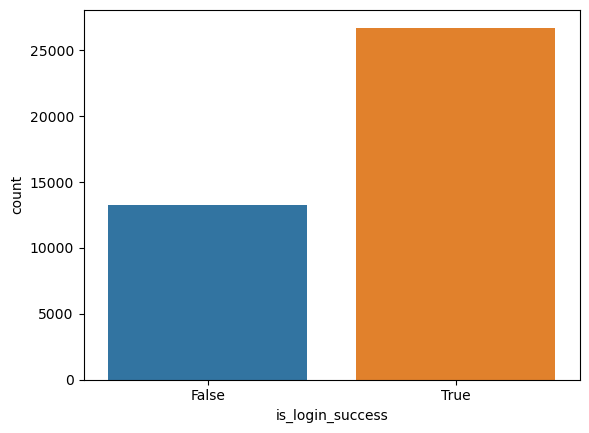
\includegraphics[width=0.5\textwidth]{contents/chapter-6/visualize_class.png}
    \caption{Presentase Target pada Dataset}
    \label{fig:visualize_target}
\end{figure}

Berdasarkan Gambar \ref{fig:visualize_target}, dapat dilihat bahwa presentase target pada dataset adalah 0.5. Dengan demikian, dapat disimpulkan bahwa dataset yang digunakan tidak seimbang. Menurut (Sun dkk., 2009) dataset yang digunakan tidak seimbang dapat menyebabkan model yang dihasilkan cenderung memprediksi kelas mayoritas. Hal ini menyebabkan akurasi yang dihasilkan lebih rendah dari yang diharapkan.





\section{Pembahasan Hasil Pengujian}
Pembahasan hasil pengujian berisi pembahasan terhadap hasil pengujian yang telah dilakukan. Pembahasan dilakukan dengan membandingkan hasil pengujian dengan spesifikasi kebutuhan yang telah ditetapkan sebelumnya. Apabila hasil pengujian sesuai dengan spesifikasi kebutuhan, maka sistem dapat dikatakan berhasil. Sebaliknya, apabila hasil pengujian tidak sesuai dengan spesifikasi kebutuhan, maka sistem dapat dikatakan gagal.
